

\begin{frame}[fragile]
\frametitle{The plasmodium data}

\begin{knitrout}\scriptsize
\definecolor{shadecolor}{rgb}{0.969, 0.969, 0.969}\color{fgcolor}\begin{kframe}
\begin{alltt}
\hlkwd{library}\hlstd{(Matrix)}
\hlkwd{load}\hlstd{(}\hlstr{"plasmodium_expression.Rdata"}\hlstd{)}
\hlkwd{dim}\hlstd{(Y)}
\end{alltt}
\begin{verbatim}
## [1] 3490   46
\end{verbatim}
\begin{alltt}
\hlkwd{head}\hlstd{(Y)[,} \hlnum{1}\hlopt{:}\hlnum{5}\hlstd{]}
\end{alltt}
\begin{verbatim}
##                TP1    TP2    TP3    TP4    TP5
## MAL13P1.100 0.4510 0.6532 1.0760 0.5515 0.4238
## MAL13P1.102 1.5320 1.8920 0.8803 1.0300 0.9328
## MAL13P1.103 0.5218 0.5213 0.5328 0.3719 0.3258
## MAL13P1.105 0.5515 0.5527 0.8627 0.4541 0.4299
## MAL13P1.107 0.5630 0.4463 1.0760 0.4035 0.2082
## MAL13P1.112 0.5390 0.5393 0.5642 0.5326 0.4469
\end{verbatim}
\end{kframe}
\end{knitrout}
\end{frame}

\begin{frame}[fragile]
\frametitle{The plasmodium data}
\framesubtitle{Gene to Gene empirical covariance}

Covariance between the 100 most variable genes.

\begin{knitrout}\scriptsize
\definecolor{shadecolor}{rgb}{0.969, 0.969, 0.969}\color{fgcolor}\begin{kframe}
\begin{alltt}
\hlstd{genes.subset} \hlkwb{<-} \hlkwd{order}\hlstd{(}\hlkwd{apply}\hlstd{(Y,}\hlnum{1}\hlstd{,var))[}\hlnum{1}\hlopt{:}\hlnum{100}\hlstd{]}
\hlkwd{image}\hlstd{(}\hlkwd{Matrix}\hlstd{(}\hlkwd{cor}\hlstd{(}\hlkwd{t}\hlstd{(Y[genes.subset, ]))),} \hlkwc{userRaster}\hlstd{=}\hlnum{TRUE}\hlstd{)}
\end{alltt}
\end{kframe}
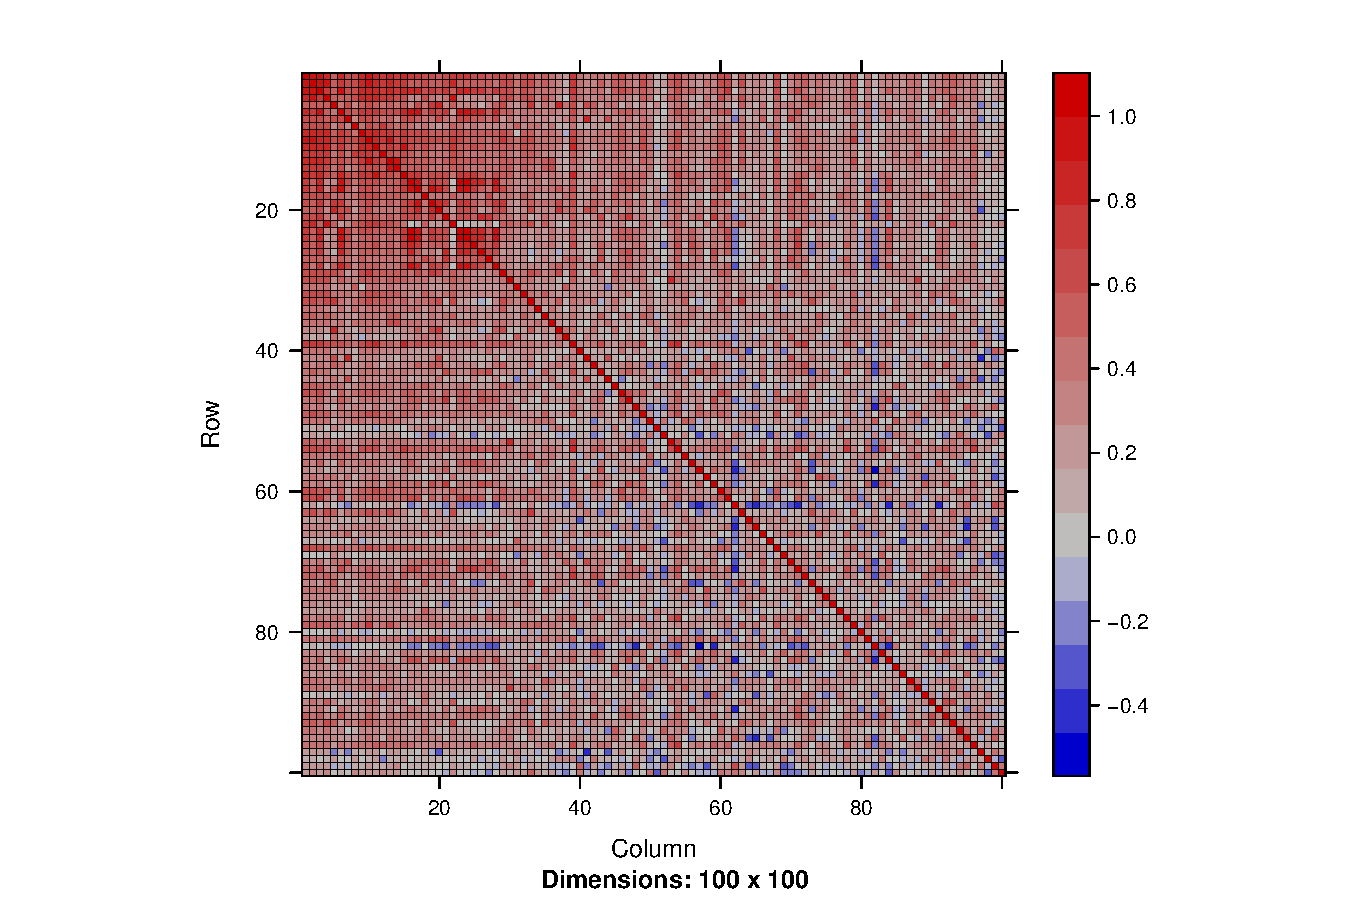
\includegraphics[width=.8\textwidth]{figures/get_plasmodium_data_fig-1} 

\end{knitrout}
\end{frame}

\begin{frame}[containsverbatim,allowframebreaks]
\frametitle{Network between the genes}
\framesubtitle{Sparse Estimation}

Regulatory network between the 100 most variable genes.

\begin{knitrout}\scriptsize
\definecolor{shadecolor}{rgb}{0.969, 0.969, 0.969}\color{fgcolor}\begin{kframe}
\begin{alltt}
\hlkwd{library}\hlstd{(huge)}
\hlstd{huge.out} \hlkwb{<-} \hlkwd{huge}\hlstd{(}\hlkwd{as.matrix}\hlstd{(}\hlkwd{t}\hlstd{(Y[genes.subset, ])),} \hlkwc{method}\hlstd{=}\hlstr{"glasso"}\hlstd{,} \hlkwc{cov.output}\hlstd{=}\hlnum{TRUE}\hlstd{)}
\end{alltt}
\begin{verbatim}
## Conducting the graphical lasso (glasso) with lossless screening....in progress:0% 
Conducting the graphical lasso (glasso) with lossless screening....in progress:9% 
Conducting the graphical lasso (glasso) with lossless screening....in progress:19% 
Conducting the graphical lasso (glasso) with lossless screening....in progress:30% 
Conducting the graphical lasso (glasso) with lossless screening....in progress:40% 
Conducting the graphical lasso (glasso) with lossless screening....in progress:50% 
Conducting the graphical lasso (glasso) with lossless screening....in progress:60% 
Conducting the graphical lasso (glasso) with lossless screening....in progress:70% 
Conducting the graphical lasso (glasso) with lossless screening....in progress:80% 
Conducting the graphical lasso (glasso)....done.                                          
\end{verbatim}
\begin{alltt}
\hlkwd{plot}\hlstd{(huge.out)}
\end{alltt}
\end{kframe}
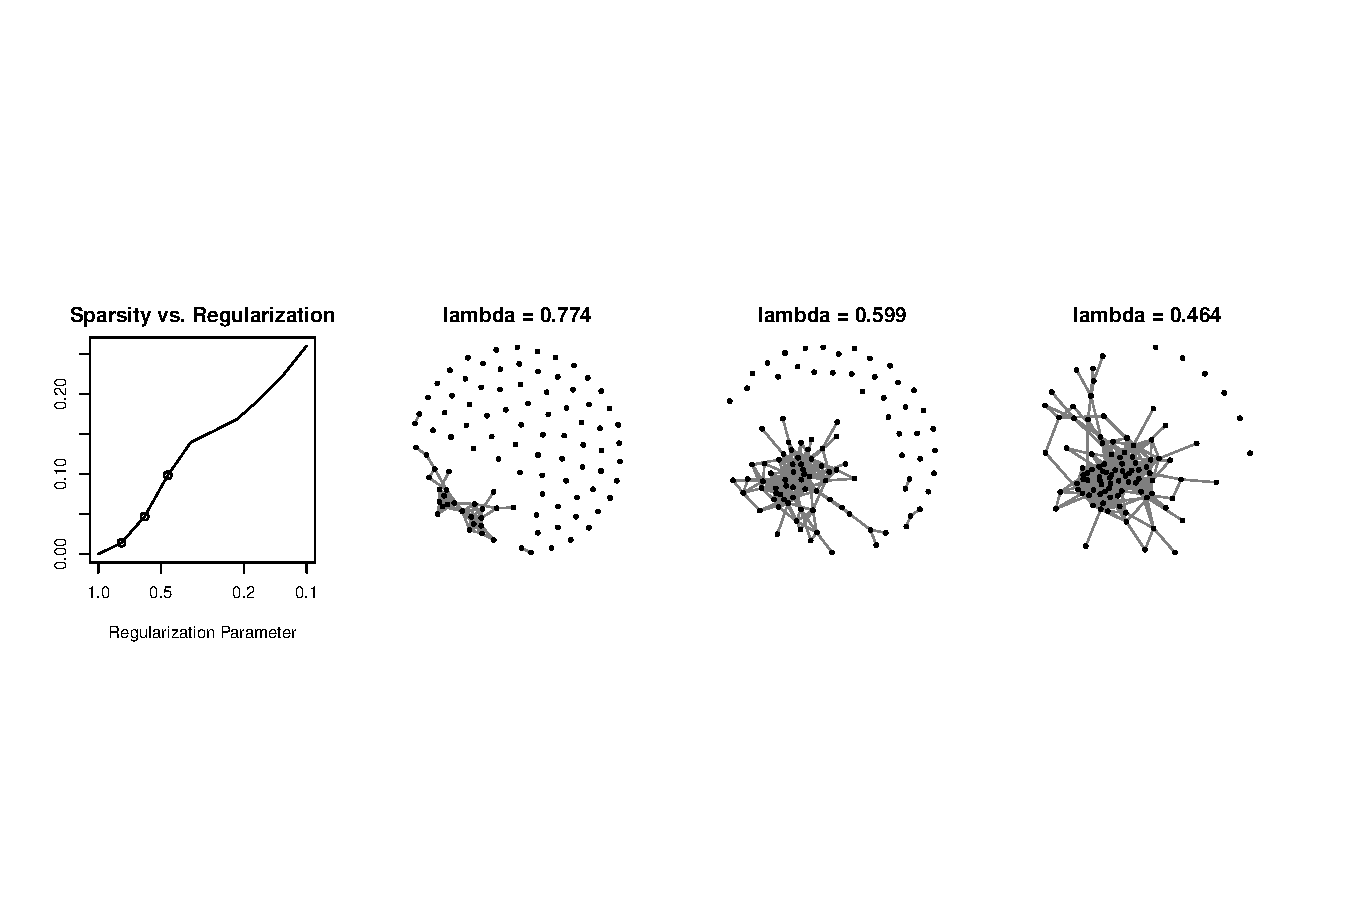
\includegraphics[width=.8\textwidth]{figures/r_show_plasmodium_glasso3-1} 

\end{knitrout}
\end{frame}

\begin{frame}[containsverbatim,allowframebreaks]
\frametitle{Network between the genes}
\framesubtitle{Inverse covariance}

\begin{knitrout}\scriptsize
\definecolor{shadecolor}{rgb}{0.969, 0.969, 0.969}\color{fgcolor}\begin{kframe}
\begin{alltt}
\hlkwd{library}\hlstd{(huge)}
\hlstd{huge.out}\hlopt{$}\hlstd{df}
\end{alltt}
\begin{verbatim}
##  [1]    0   71  233  488  693  763  836  963 1110 1289
\end{verbatim}
\begin{alltt}
\hlkwd{image}\hlstd{(}\hlkwd{Matrix}\hlstd{(huge.out}\hlopt{$}\hlstd{icov[[}\hlnum{3}\hlstd{]]))}
\end{alltt}
\end{kframe}
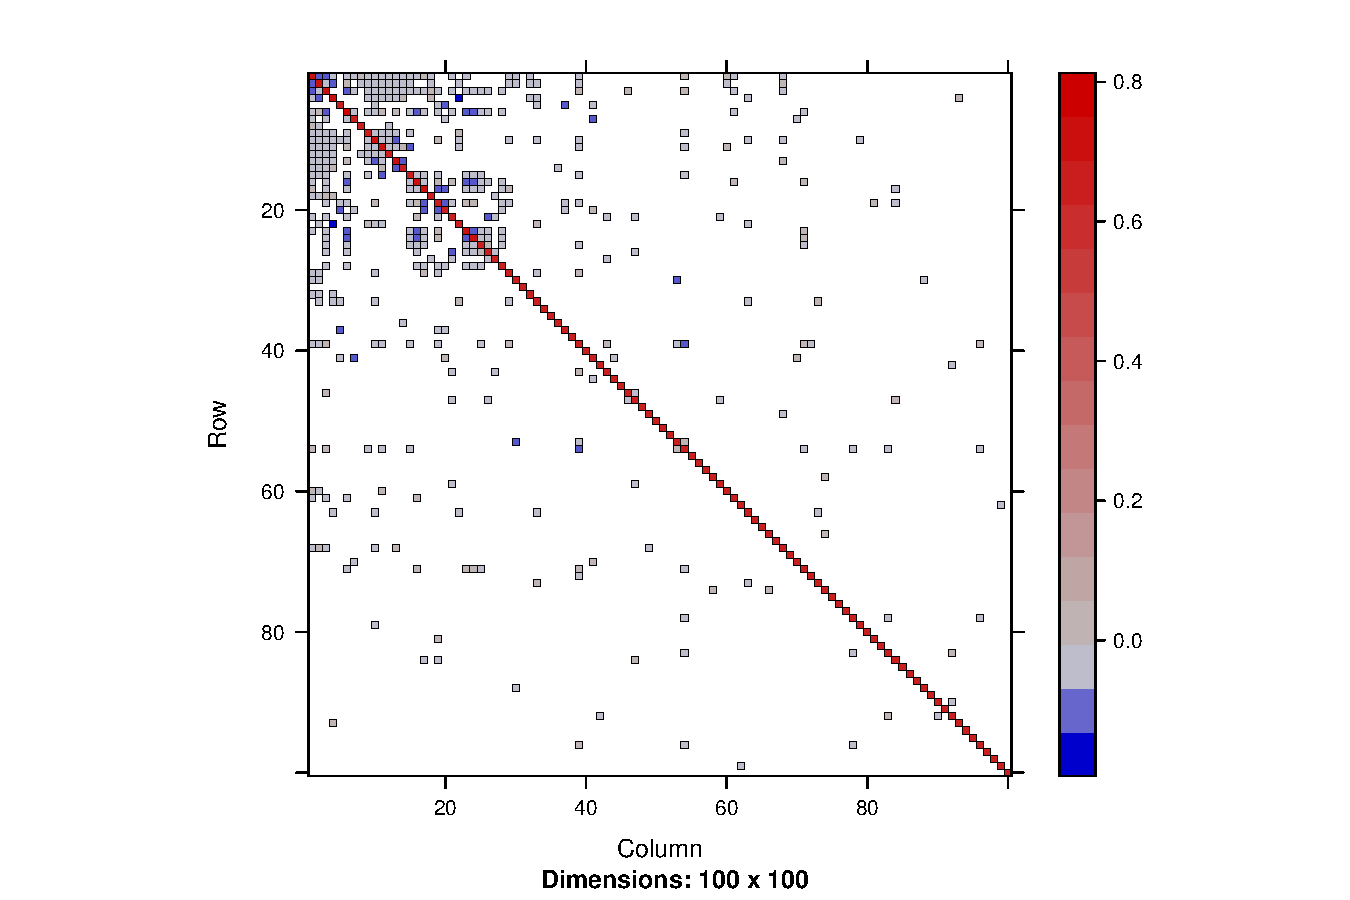
\includegraphics[width=.8\textwidth]{figures/r_show_plasmodium_glasso4-1} 

\end{knitrout}
\end{frame}

\begin{frame}[fragile]
\frametitle{The plasmodium data}
\framesubtitle{Covariance between conditions}

\begin{knitrout}\scriptsize
\definecolor{shadecolor}{rgb}{0.969, 0.969, 0.969}\color{fgcolor}\begin{kframe}
\begin{alltt}
\hlkwd{image}\hlstd{(}\hlkwd{Matrix}\hlstd{(}\hlkwd{cor}\hlstd{(Y)))}
\end{alltt}
\end{kframe}
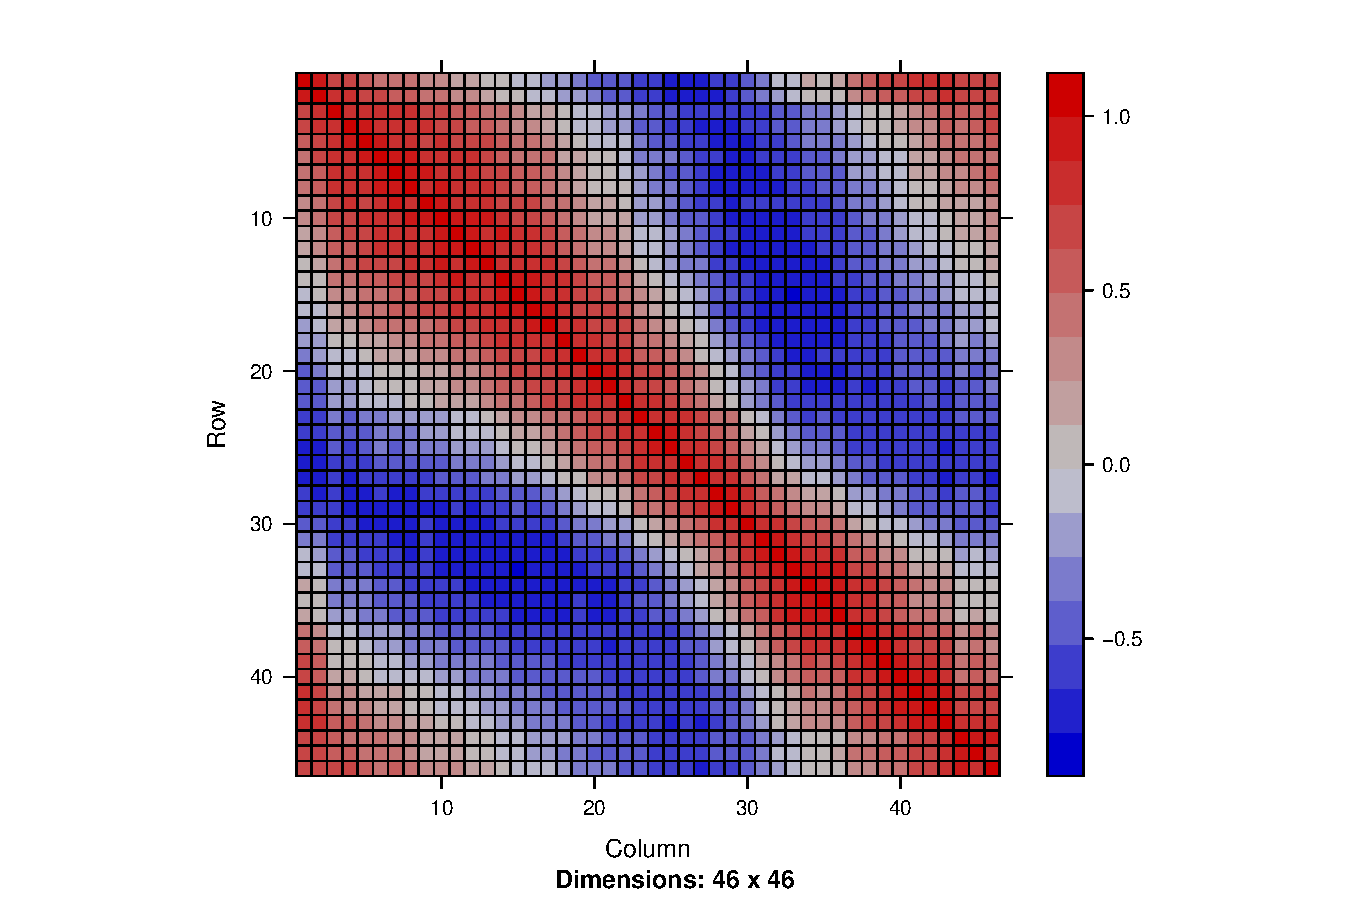
\includegraphics[width=.8\textwidth]{figures/get_plasmodium_data_fig_cond-1} 

\end{knitrout}
\end{frame}

\begin{frame}[containsverbatim]
\frametitle{Covariance structure between the conditions}
\framesubtitle{Sparse Estimation}

\begin{knitrout}\scriptsize
\definecolor{shadecolor}{rgb}{0.969, 0.969, 0.969}\color{fgcolor}\begin{kframe}
\begin{alltt}
\hlkwd{library}\hlstd{(huge)}
\hlstd{huge.out} \hlkwb{<-} \hlkwd{huge}\hlstd{(}\hlkwd{as.matrix}\hlstd{(Y),} \hlkwc{method}\hlstd{=}\hlstr{"glasso"}\hlstd{,} \hlkwc{cov.output}\hlstd{=}\hlnum{TRUE}\hlstd{)}
\end{alltt}
\begin{verbatim}
## Conducting the graphical lasso (glasso) with lossless screening....in progress:0% 
Conducting the graphical lasso (glasso) with lossless screening....in progress:9% 
Conducting the graphical lasso (glasso) with lossless screening....in progress:19% 
Conducting the graphical lasso (glasso) with lossless screening....in progress:30% 
Conducting the graphical lasso (glasso) with lossless screening....in progress:40% 
Conducting the graphical lasso (glasso) with lossless screening....in progress:50% 
Conducting the graphical lasso (glasso) with lossless screening....in progress:60% 
Conducting the graphical lasso (glasso) with lossless screening....in progress:70% 
Conducting the graphical lasso (glasso) with lossless screening....in progress:80% 
Conducting the graphical lasso (glasso)....done.                                          
\end{verbatim}
\begin{alltt}
\hlstd{sel.out}  \hlkwb{<-} \hlkwd{huge.select}\hlstd{(huge.out)}
\end{alltt}
\begin{verbatim}
## Conducting extended Bayesian information criterion (ebic) selection....done
\end{verbatim}
\end{kframe}
\end{knitrout}
\end{frame}

\begin{frame}[containsverbatim]
\frametitle{Covariance structure between the conditions}
\framesubtitle{Sparse Estimation}

\begin{knitrout}\scriptsize
\definecolor{shadecolor}{rgb}{0.969, 0.969, 0.969}\color{fgcolor}\begin{kframe}
\begin{alltt}
\hlkwd{image}\hlstd{(sel.out}\hlopt{$}\hlstd{opt.cov)}
\end{alltt}
\end{kframe}
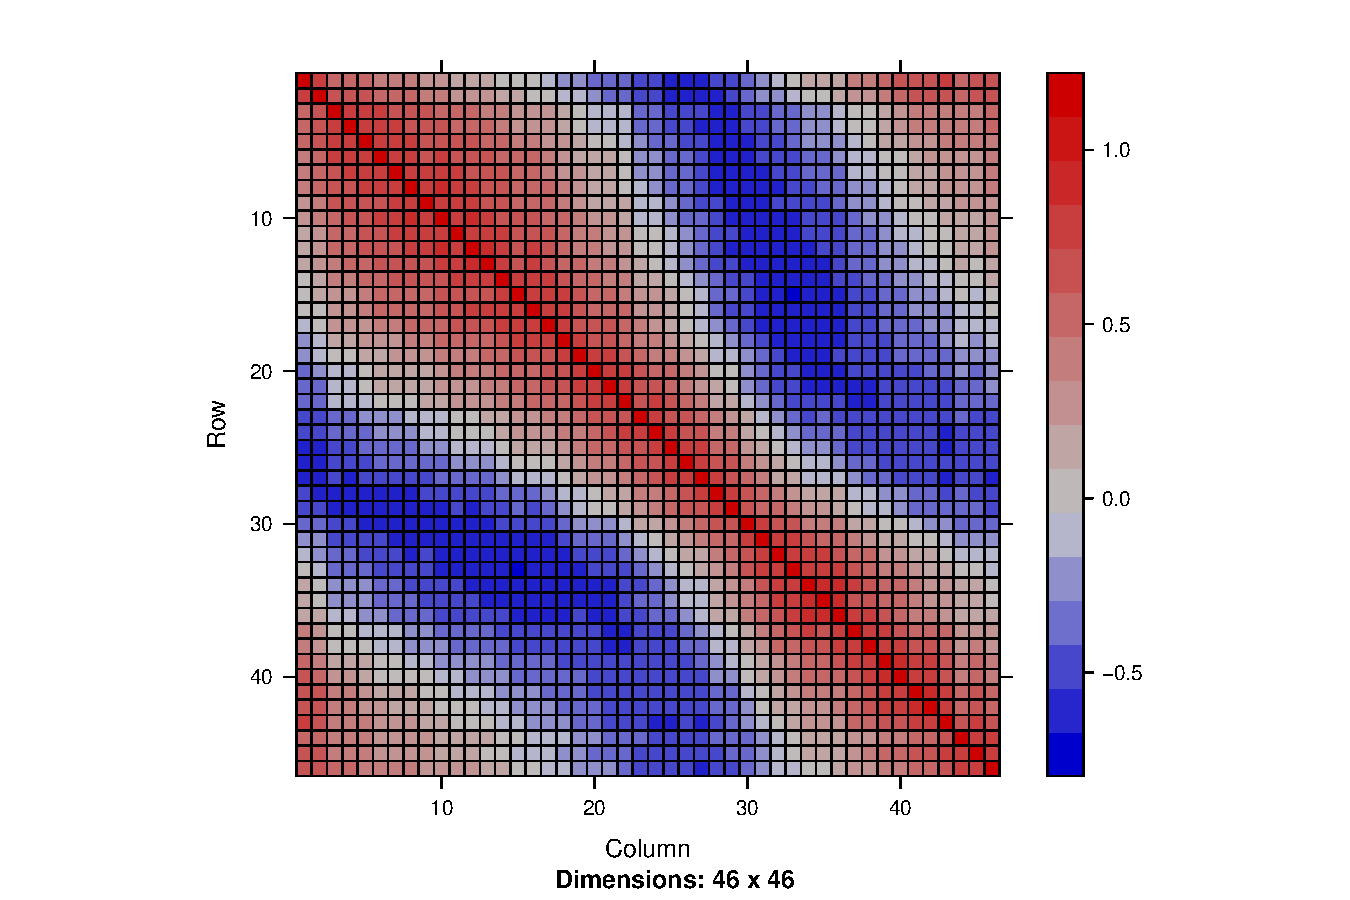
\includegraphics[width=.8\textwidth]{figures/r_get_plasmodium_glassob-1} 

\end{knitrout}
\end{frame}

\begin{frame}[containsverbatim,allowframebreaks]
\frametitle{Covariance structure between the conditions}
\framesubtitle{Sparse Estimation of the inverse covariance}

\begin{knitrout}\scriptsize
\definecolor{shadecolor}{rgb}{0.969, 0.969, 0.969}\color{fgcolor}\begin{kframe}
\begin{alltt}
\hlkwd{sum}\hlstd{(}\hlkwd{abs}\hlstd{(sel.out}\hlopt{$}\hlstd{opt.icov)} \hlopt{!=} \hlnum{0}\hlstd{)}
\end{alltt}
\begin{verbatim}
## [1] 760
\end{verbatim}
\begin{alltt}
\hlkwd{ncol}\hlstd{(sel.out}\hlopt{$}\hlstd{opt.icov)} \hlopt{**} \hlnum{2}
\end{alltt}
\begin{verbatim}
## [1] 2116
\end{verbatim}
\begin{alltt}
\hlkwd{image}\hlstd{(sel.out}\hlopt{$}\hlstd{opt.icov)}
\end{alltt}
\end{kframe}
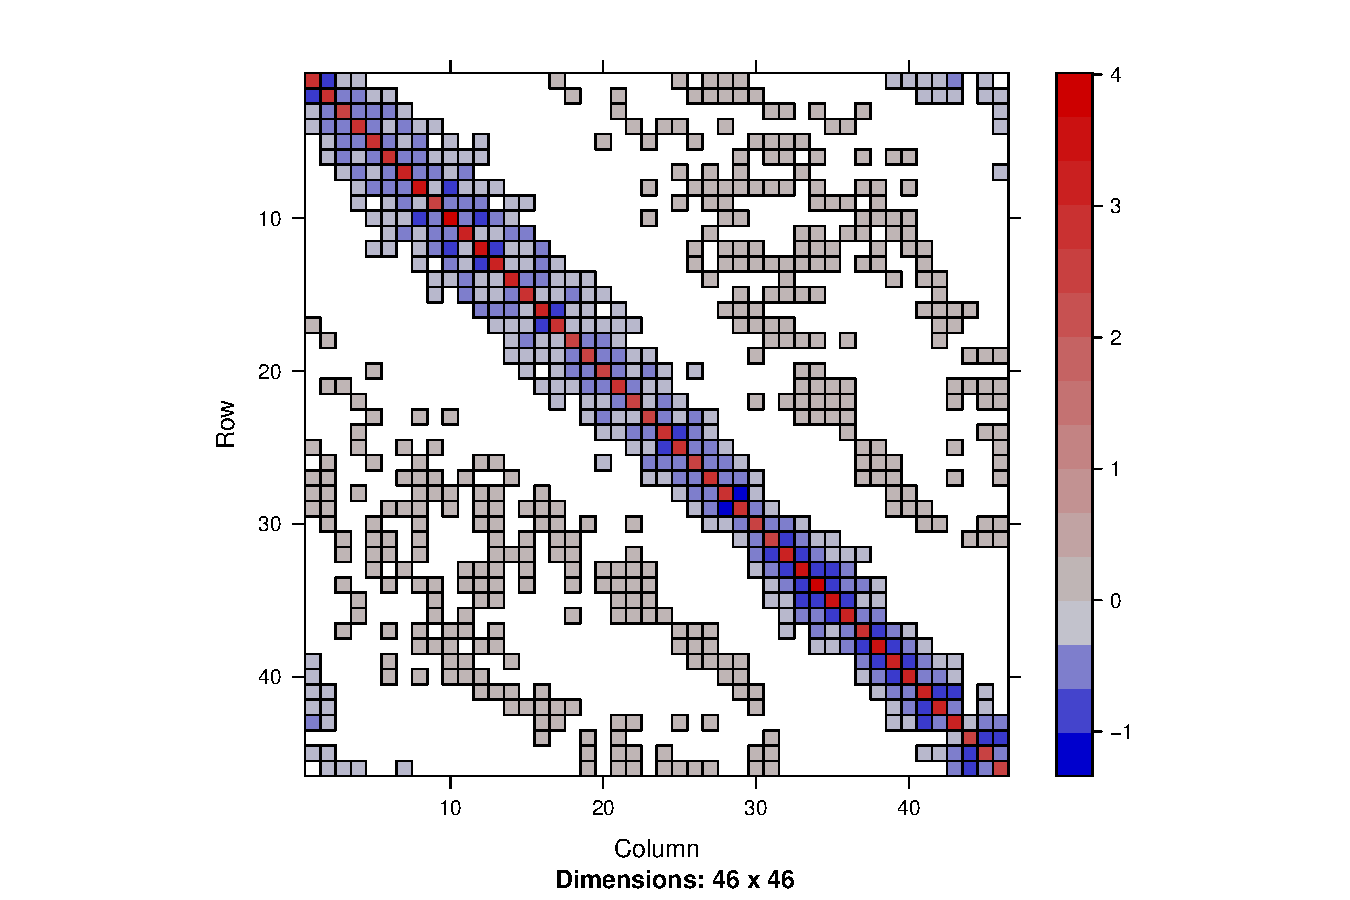
\includegraphics[width=.8\textwidth]{figures/r_show_plasmodium_glasso-1} 

\end{knitrout}

\end{frame}

\begin{frame}[containsverbatim,allowframebreaks]
\frametitle{Covariance structure between the conditions}
\framesubtitle{Associated network}

\begin{knitrout}\scriptsize
\definecolor{shadecolor}{rgb}{0.969, 0.969, 0.969}\color{fgcolor}\begin{kframe}
\begin{alltt}
\hlkwd{plot}\hlstd{(huge.out)}
\end{alltt}
\end{kframe}
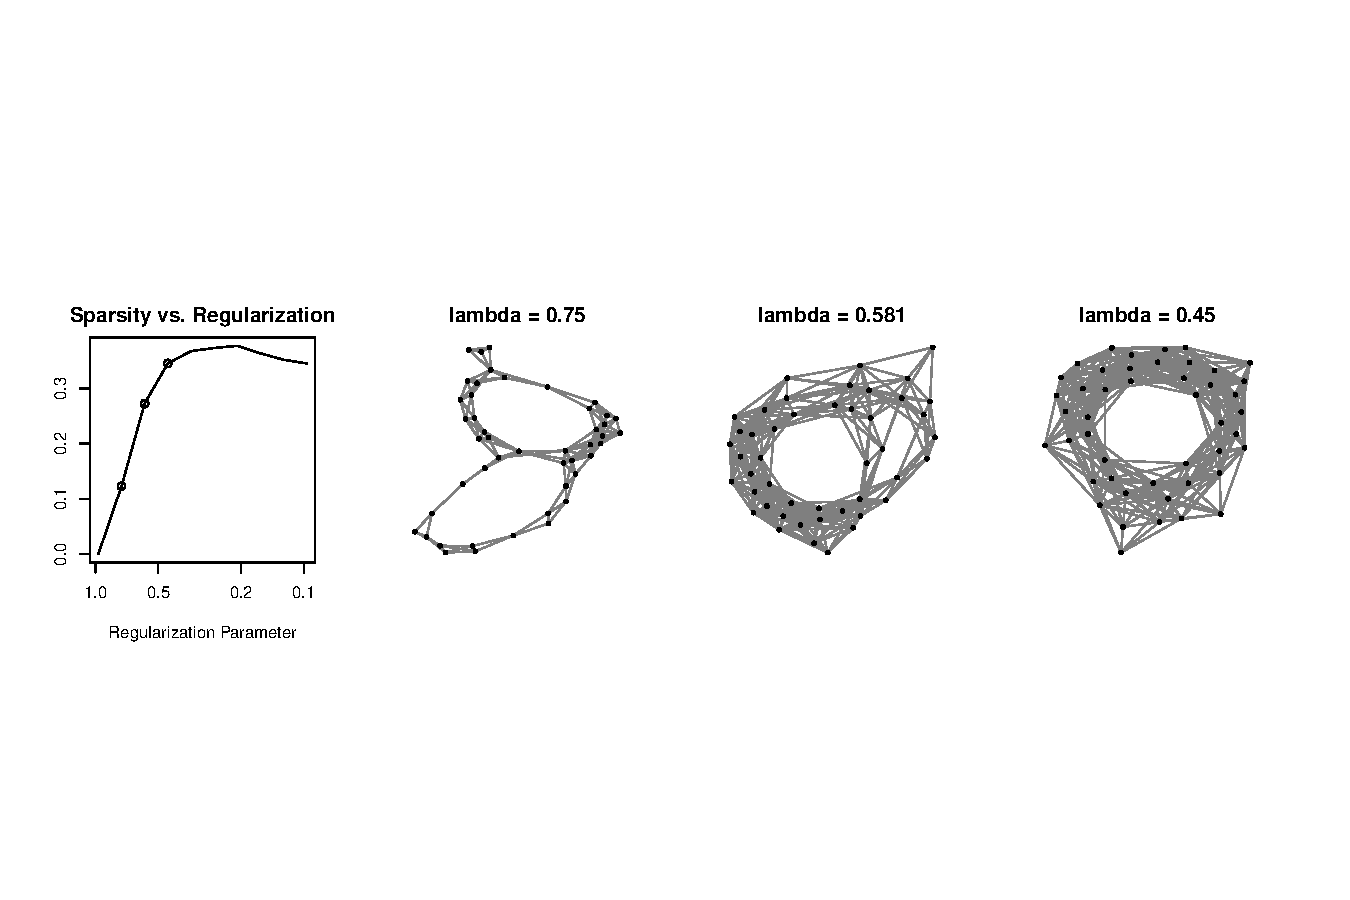
\includegraphics[width=.8\textwidth]{figures/r_show_plasmodium_glasso2-1} 

\end{knitrout}

\end{frame}

